% !TEX root=../main.tex

\chapter{Validating the automatic Pandora-based reconstruction}\label{chap:methods}

The Pandora-based event reconstruction pipeline, as described in \autoref{sec:TPC_reco_gen}, has been --- and continues to be --- central to the physics analyses conducted with the ICARUS detector. Its use across the LArTPC community ensures it is a set of tools that is actively developed. Any improvement made by each collaboration sharing this tool is thus an improvement that can be exploited on all the experiments that use it.

The Pandora framework in ICARUS employes the same structure inherithed from the MicroBooNE collaboration, shared also with the SBND experiment. Especially important for the success of the SBN programme is the fact that the reconstruction is nearly identical for both the near and the far detector, in order to make systematic uncertainties related to the reconstruction as less relevant as possible. 

Recent efforts were made to better align the Pandora reconstruction paths between ICARUS and SBND, with the inclusion of shower-targeted algorithms, aiming at refining the shower clusters. Moving in the same direction, this work focuses on the implementation of a set of tools that enable the use of true Monte Carlo information to alter the reconstruction output of the different stages. This comprehensive set of tools has already been tested and used in the context of the SBND reconstruction, as well as for other Pandora-based reconstruction pipelines \cite{Mawby:2023nws}. 

These tools allow to disect the impact of each step of the Pandora reconstruction by altering the reconstructed objects using the true Monte Carlo information. Using these methods provide for validation tools of the event reconstruction chain. 

However, developing reconstruction improvement in vacuum is both difficult and do not provide all the times a clear quantification of the impact made.
So, I instead targeted my studies toward a precise analysis to be able to identify pain points of the reconstruction chain. 

The ICARUS collaboration, using the collected data of the second physics data taking campaign, performed as a standalone one-detector campaign, is moving towards a first oscillation analysis, preliminary to the two-detector oscillation analysis expected with the data collected by the SBN programme. This preliminry analysis is targeted at studying the muon neutrino disappearance channel to project sensitivity curves onto the $(\Delta m^2, \sin^22\theta_{\PGm\PGm})$. 

The $\PGnGm$-disappearance analysis ongoing within the collaboration uses a precise event topology, namely the muon neutrino charged current quasi elastic topology, with one muon in the final state, any number greater than ero of protons, and requires zero electromagnetic showers (both from electrons and from photons) and zero charged pions. This selection is reffered to as $\PGnGm$CC N$\Pp$ QE \cite{particles8010018, arteroponsStudyReconstructionNuMuCC}.  

\section{Data sample and selection}

The $1\PGm N\Pp$ event topology used in the muon neutrino disappearance study are selected automatically using a thorougly tuned and tested selection procedure \cite{particles8010018}. I will now delve a little bit inside the details of the event selection procedure, highlighting the decisions that went behind the variables cuts. 

\paragraph{CRT-PMT match} Exploiting the CRT-PMT match performed in the event reconstruction, non-contained neutrinos or cosmic-ray particles are rejected. The cut searches for coincidences in the \SI{150}{\ns} gate between CRT hits and an optical flash. All optical flashes are looked into the \qtyrange{0}{1.6}{\us} spill gate, and only the spills that have no CRT hit associated are kept. This first contributes to reducing the huge amount of cosmic ray interactions in the detector, thus slightly improving on the selection purity. 

\paragraph{Optical flash barycenter match} The light information coming from the PMTs is also used to improve the selection by exploiting its 3D information. Using the light from the triggering PMT flash, the barycenter of the light hit is computed. The barycenter is computed as the mean of optical hits, weighted on the signal integral on each optical hit, \begin{equation}
    \vec{x} = \frac{\sum_i \vec x_i \cdot \mathrm{PE}_i}{\sum_i \mathrm{PE}_i}.  
\end{equation} Here $\vec x_i$ represent the position of the PMT producing the $i$-th, with a signal integral of $\mathrm{PE}_i$ photo-electrons collected by the $i$-th photomultiplier. This position information is used to reject all slices whose charged $z$-barycenter was more than \SI{1}{\m} away from the light $z$-barycenter. This choice was made considering the best cut to minimise he contamination from other interaction types, as well as maximise the selection efficiency. 

\paragraph{Vertex and tracks containment} Two basic selection cuts are then applied to the vertices and track in the interaction selected by the first two cuts. The vertex is required to be insde the fiducial volume (requiring more than \SI{25}{\cm} apart from the lateral TPC walls and 30/\SI{50}{\cm} from the upstream/downstream walls) of the ICARUS detector, defined in \cite{arteroponsStudyReconstructionNuMuCC}, whereas all the tracks inside the interaction are required to be contained in the active volume of the TPC within \SI{5}{\cm} from all the sides. This request ensures that the PID score described in \eqref{eq:PID} can be computed and provides for a great separation between different particle species. 

The interactions that pass these preliminary quality cuts are then analysed by term of particle content, so each particle in the interaction is classified as such, and interactions with one muon, $N$ protons (with $N\geq1$), zero charged pions and zero showers are selected. I will now define the variable cuts applied to identify each particle species. 

\paragraph{Muon identification} The muon track is identified as the reconstructed longest particle fulfilling the following set of requests \begin{itemize}
    \item It should be tagged as a primary particle, so its parent should be the neutrino associated with the interaction vertex. 
    \item It should be identified as a track-like object. The BDT implemented at the end of the Pandora reconstruction chain performs a topological classification of  each object inside the interaction, assigning a ``trackscore'' value between zero and one. The more an object is ``track-like'', the closer to one this score should be. The requirement for muons is a trackscore $\geq 0.5$. 
    \item The reconstructed muon length should be greater than \SI{50}{\cm}
    \item The track starting point should be less than \SI{10}{\cm} from the interaction vertex.
    \item Finally, the PID information is considered. This requires the $\chi^2$ value to be $\chi^2_\PGm < 30$ (using the $\dv*{E}{x}$ energy loss under the hypothesis that the object is a muon) and also $\chi^2_\Pp > 60$ (using the $\dv*{E}{x}$ energy loss under the hypothesis that the object is a proton). 
\end{itemize} In the reconstructed interaction, only one muon is required, passing this selection. 

\paragraph{Proton identification} The identification of the proton follows similar cuts as for the muon, with less strict selections \begin{itemize}
    \item The requirement to be tagged as a primary particle is the same as that which was present for muons.
    \item The track score, by looking at its distribution, was found to be slightly shifted to lower values, so a lower threshold is required of $\geq 0.45$. 
    \item It is required that primary protons should have a length greater than \SI{2.3}{\cm}, so a request of a minimum of \SI{50}{\mega\electronvolt} of deposited energy is required, which corresponds to a proton length of \SI{2.3}{\cm}. 
     \item The track starting point should be less than \SI{10}{\cm} from the interaction vertex.
     \item PID is then considered, requiring that $\chi^2_\Pp < 100$. 
\end{itemize} Any number greater than zero of protons is required in the $\PGnGm$CC Np QE selection. 

\paragraph{Pion identification and rejection} Pions are identified using very identical selection cuts as protons, with the only exception of requiring $\chi^2_\Pp > 100$, and a deposited energy of \SI{25}{\mega\electronvolt}. If one or more pions are identified within a certain slice, the slice gets rejected. 

\paragraph{Electromagnetic shower identification} Electromagnetic showers are identified by means of trackscore alone; everything with a value lower than 0.5, which is not classified as a proton (so $\chi^2_\Pp > 100$, among other cuts), is identified as an electromagnetic shower. If more than zero showers are reconstructed and identified  in a given slice, the slice gets rejected. 

The performances of the aforementioned selection have been  evaluated \cite{artero_pons_2024_13841852, particles8010018} by computing the selection efficiency and selection purity, respectively \begin{equation}
    \begin{aligned}
        \mathrm{Efficiency} &\equiv \frac{\text{Selected signal}}{\text{True signal}} = \SI{49}{\percent} \\
        \mathrm{Purity} &\equiv \frac{\text{Selected signal}}{\text{All selected}} = \SI{84}{\percent}
    \end{aligned}
\end{equation} The selection, with minor changes related to the differences in the reconstruction paradigm, is applied also to data reconstructed with the SPINE chain, described in \autoref{sec:SPINE}. Using this different reconstruction paradigm, the efficiency and purity values obtained are, respectively, of $\sim\SI{75}{\percent}$ and $\sim\SI{80}{\percent}$. 

Parallel to both reconstruction chains, the efficiencies and purities were validated by visual scan using a small data sample ($\sim\SI{2e18}{POT}$), confirming the aforementioned values for both analyses. 

\section{\emph{Cheating} the Pandora reconstruction} 

The modular structure of the Pandora reconstruction allows for great flexibility of the tools and algorithms involved in the reconstruction. As described in \autoref{sec:TPC_reco_gen}, and pictured in \autoref{fig:PandoraFastReco}, \ref{fig:PandoraCosmic} and \ref{fig:PandoraNeutrino}, a sequence of multiple algorithms is applied to the hit objects, resulting in reconstructed objects. The steering of the Pandora reconstruction chain is performed by XML configuration files where each algorithm is declared and configured. An example of the steering algorithm for the TrackClusterCreation algorithm, present in both the PandoraFastReco, PandoraCosmic and PandoraNeutrino paths is displayed below.

\begin{lstlisting}[style=xmlstyle]
<pandora>
    ...
    <!-- TwoDReconstruction -->
    <algorithm type = "LArClusteringParent">
        <algorithm type = "LArTrackClusterCreation" description = "ClusterFormation"/>
        <InputCaloHitListName>CaloHitListU</InputCaloHitListName>
        <ClusterListName>ClustersU</ClusterListName>
        <ReplaceCurrentCaloHitList>true</ReplaceCurrentCaloHitList>
        <ReplaceCurrentClusterList>true</ReplaceCurrentClusterList>
    </algorithm>
    ...
</pandora>
\end{lstlisting}

This modular approach of the Pandora topological event reconstruction can be exploited to allow an algorithm to be replaced with a functionally identical algorithm, which, instead of relying on the actual tools to perform the reconstruction task, uses the underlying Monte Carlo information. This approach, developed as part of the Pandora reconstruction framework, is in this thesis referred to as ``\emph{cheating}'' of the reconstruction. The powerfulness of this concept has been shown already with reconstruction studies in other experiments, where it is employed to pinpoint the ``failure points'' of the topological event reconstruction and understand the ceiling performances of the Pandora reconstruction, assuming certain steps of the reconstruction are perfect \cite{Mawby:2023nws, Mawby:2025_FCCee, Nguyen:2023_cheatingPandora}. 

In practical terms, cheating one or multiple algorithms involves replacing the corresponding algorithm in the steering XML configuration file with the respective cheating counterpart. For example, the configuration shown above, guiding the creation of two-dimensional clusters on the $u$ view, is replaced by the CheatingClusterCreation algorithm, which performs the cheating of the cluster creation (which is the first step of both the PandoraCosmic and PandoraNeutrino paths, see \autoref{fig:PandoraCosmicNeutrino}), listed below 

\begin{lstlisting}[style=xmlstyle]
<pandora>
    ...
    <algorithm type = "LArClusteringParent">
        <algorithm type = "LArCheatingClusterCreation" description = "ClusterFormation">
            <!-- Cheating specific configurations -->
            <CollapseToPrimaryMCParticles>false</CollapseToPrimaryMCParticles>
            <MCParticleListName>Input</MCParticleListName>
        </algorithm>
        <InputCaloHitListName>CaloHitListU</InputCaloHitListName>
        <ClusterListName>ClustersU</ClusterListName>
        <ReplaceCurrentCaloHitList>false</ReplaceCurrentCaloHitList>
        <ReplaceCurrentClusterList>true</ReplaceCurrentClusterList>
    </algorithm>
    ...
</pandora>
\end{lstlisting}

The action of cheating one algorithm can be seen as making the cheated step of the reconstruction have a perfect success rate. Cheating different steps takes into account the action of each step of the reconstruction. The next paragraphs are entirely dedicated to delving into the details of how cheating is applied to different algorithms of the Pandora reconstruction chain. 

\subsection{Two-dimensional clustering}

All three paths employed in the ICARUS event reconstruction share a set of algorithm, the firsts being involved with the clustering of the hits on each of the three readout planes. Cheating this step is pretty straightforward. Using simulated data, the hits on the three $u$, $v$ nd $w$ views have associated with them a value called ``MCWeight'', expressing how much a given MCParticle in the interaction is related to the simulated deposited hit on the readout plane. Using the MCWeights it is possible for the hits to get mapped to the respective MCParticle, and thus build cluster on each of the 2D planes using the simulation true information. The effect for tracks, like muons and protons, is noticeable but yet not striking, whereas the effect for electromagnetic showers is huge, since this approach does not just cluster continuous lines of hits, but, using MC association to the true underlying event, can group together hits in more complex topologies. Hence, the presence of the CheatingClusterCreation algorithm makes some of the subsequent algorithms, used in the nominal (i.e. not ``cheated'') reconstruction chain, irrelevant. 

As most of the algorithms used within the Pandora framework, itis highly customizable, allowing only one view of the three to be cheated, and also allowing only one type of particle to have its cluster created by using true information. Due to the ICARUS geometry, and the details discussed in \autoref{sec:ICARUS_T600} (illustrated in \autoref{fig:i2_c_planes_wirepitch_detail}), the first option is only possible considering either the induction-1 plane and/or the induction-2 and collection plane together.

\autoref{fig:CheatingClusterCreation} illustrate the action of the cheated algorithm, showing the clusters created after a single pass of the TrackClusterCreation algorithm and the cluster created by the CheatingClusterCreation algorithm. The effect, thought very subtle for track particles, which are the star of the $\PGnGm$CC QE Np selection in use, is noticeable especially in the cluster refinements. Less noisy hits are clustered together, resulting in an overall improvement in the downstream reconstruction of the 3D particles. 

\begin{figure}
    \centering
    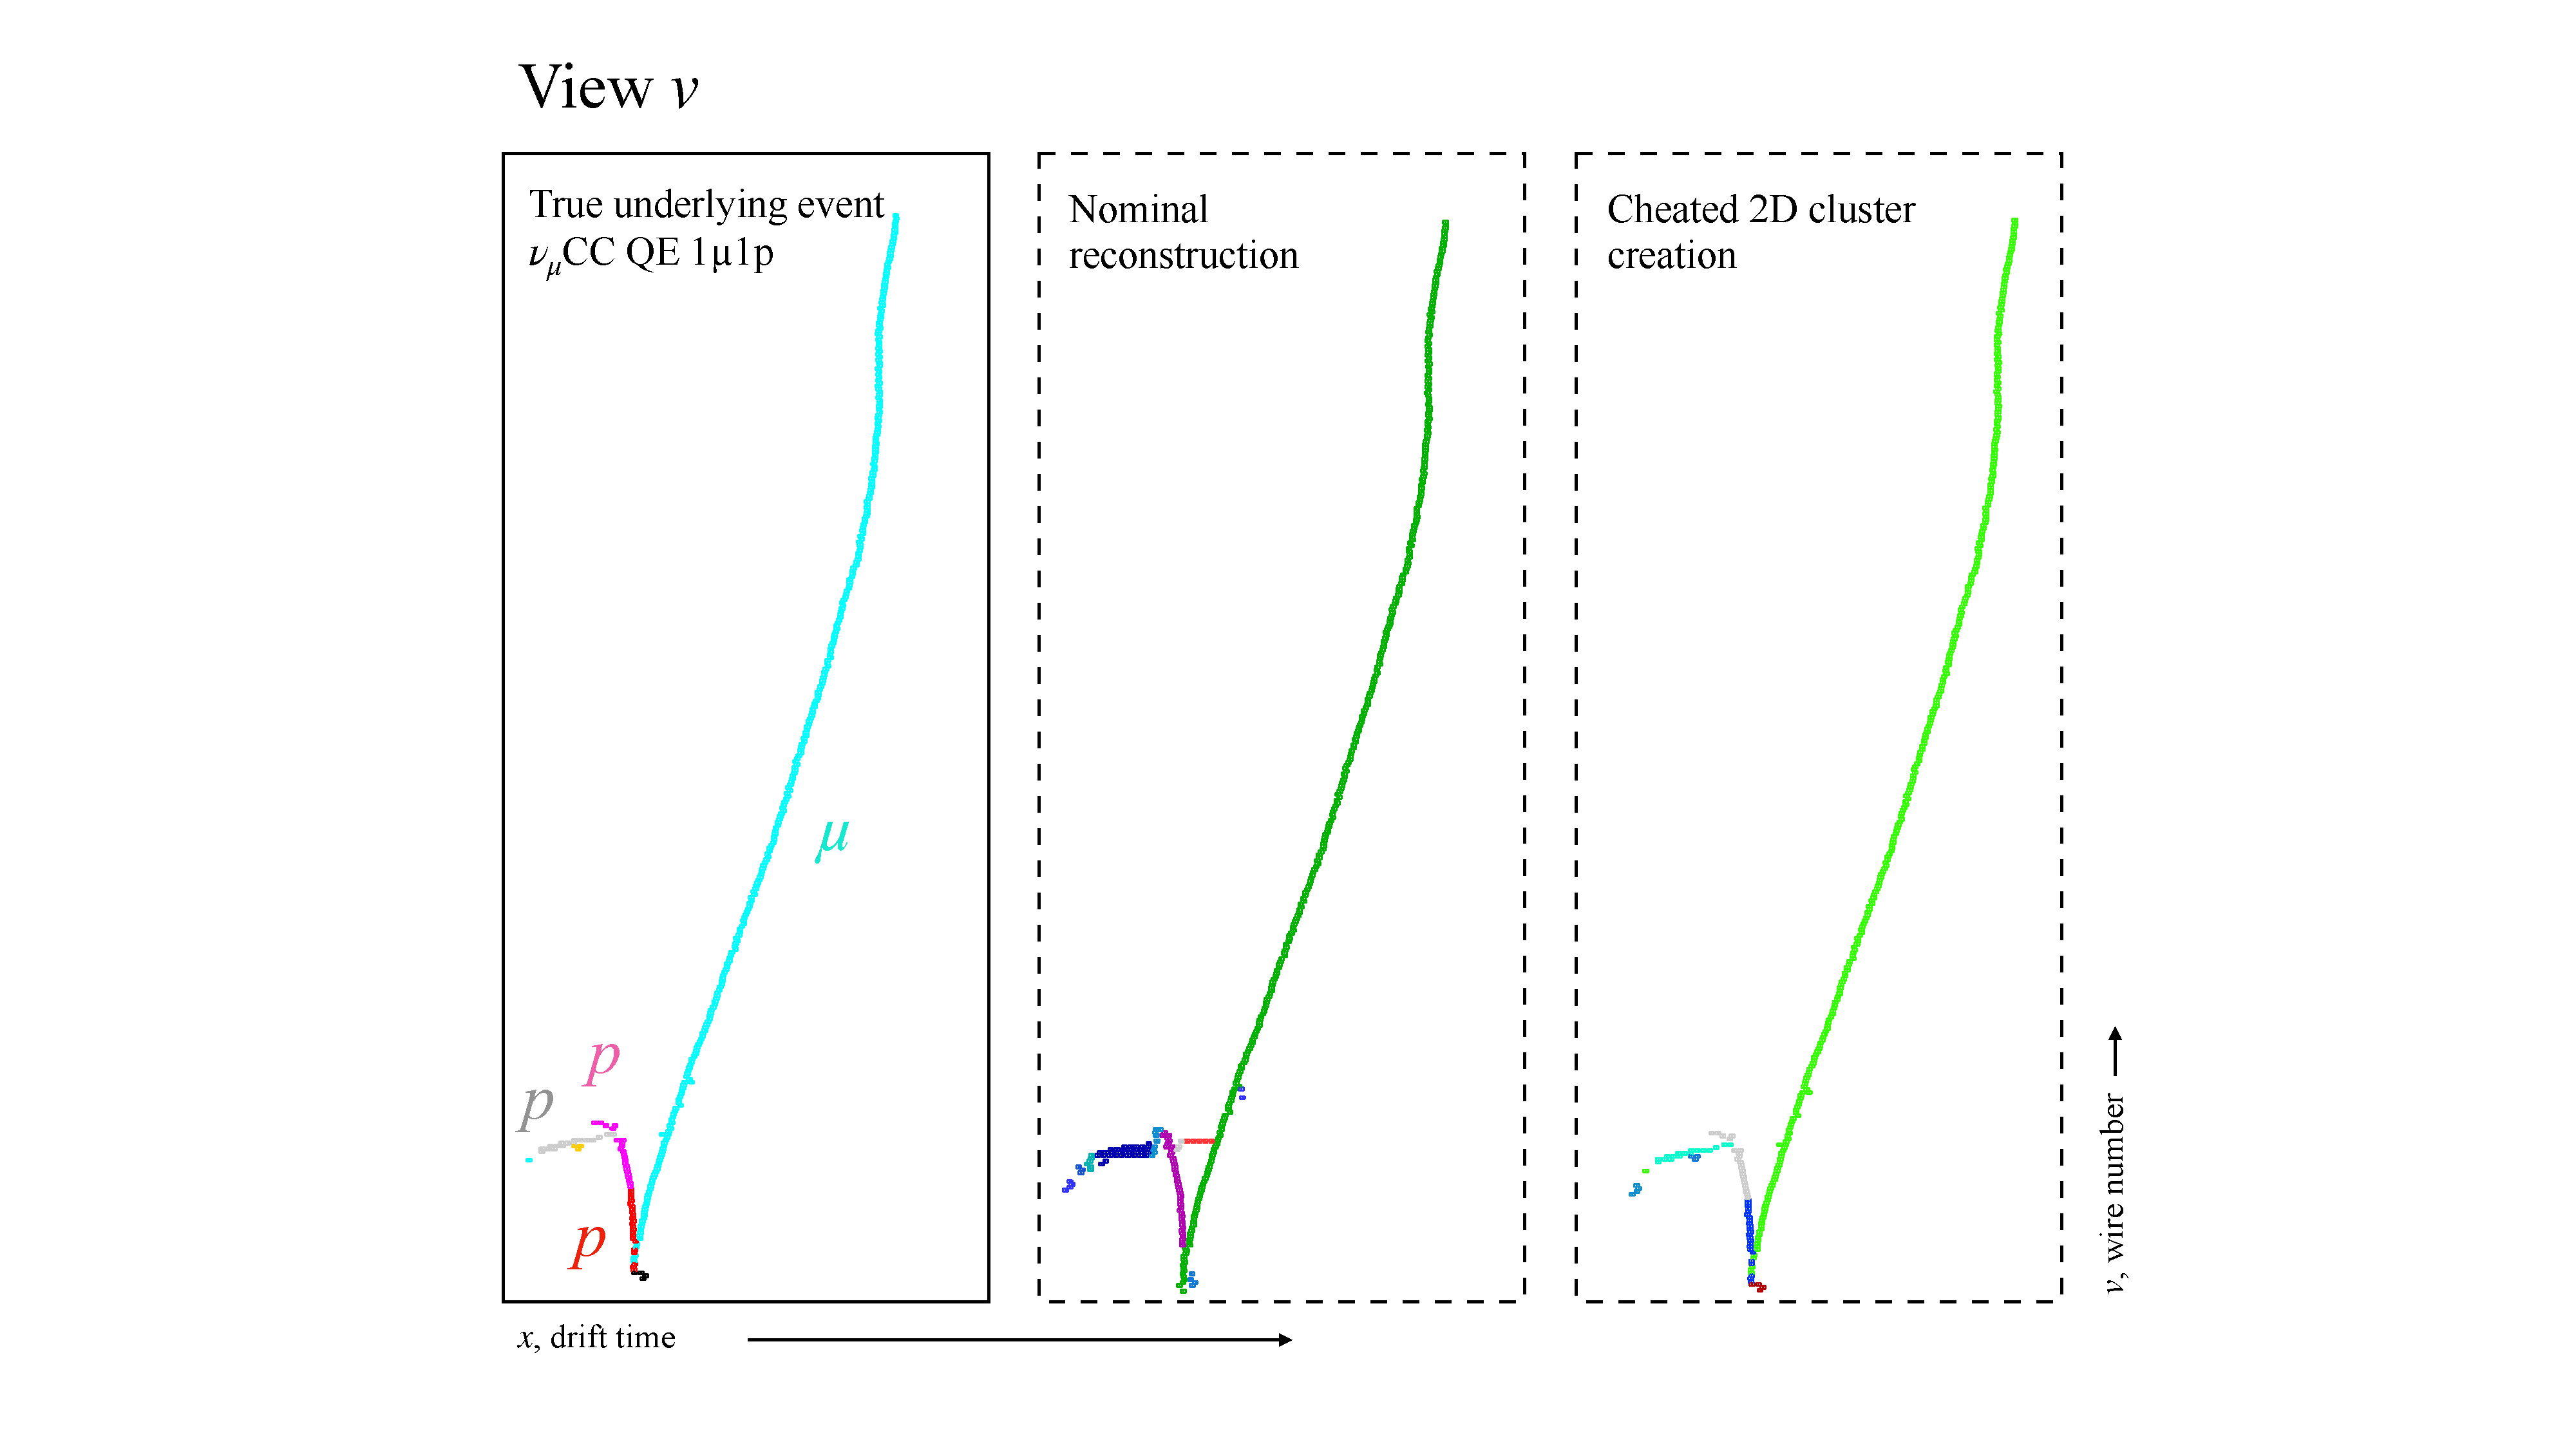
\includegraphics[width=0.85\linewidth, trim={12cm 0 11cm 0}, clip]{pandora/chapter_4/cluster2D.pdf}
    \caption[CheatingClusterCreation versus TrackClusterCreation algorithm]{Illustation of the effect of the CheatingClusterCreation algorithm, with a $1\PGm1Pp$ event. The amount of noise in the proton daughter particles is greater, resulting in a lower hit purity, whereas the cheated clusters show a better refinement. The center panel shows the true underlying neutrino interaction, where the secondary protons created from the reinteraction of the primary proton are illustrated. }
    \label{fig:CheatingClusterCreation}
\end{figure}

To assess that the effect of the CheatingClusterCreation algorithm was as expected, a downstream metric has to be selected. Given that the TrackClusterCreation algorithm objective is to assign the correct hits to the respective track in each plane, two valid metrics are the \emph{hit completeness} and \emph{hit purity} scores. Given the hits on the readout plane, its possible to define the MC matched hits, that are the hits that are associated with the MCParticle andh are also associated by Pandora to the PFParticle \begin{equation}
    \mathrm{Matched\ hits} \equiv \mathrm{hits_{MCParticle} \cap hits_{PFParticle}}.
\end{equation} Looking at the illustration in \autoref{fig:hit_pur_eff}, two particles are present. The reconstructed PFParticle $j$ has a total of seven hits associated by the Pandora reconstruction, whereas PFParticle $k$ has six; The true MCParticle $j$ has nine hits, and $k$ has four. So for Particle $j$ the matched hits are seven, and for $k$ are four. We can therefore define the hit purity and hit completeness as \begin{equation}
    \mathrm{Hit\ purity} \equiv \frac{\mathrm{Matched\ hits}}{\mathrm{hits_{PFParticle}}}, 
\end{equation} and \begin{equation}
    \mathrm{Hit\ completeness} \equiv \frac{\mathrm{Matched\ hits}}{\mathrm{hits_{MCParticle}}}. 
\end{equation} So, in the example in \autoref{fig:hit_pur_eff}, we have a purity of \SI{100}{\percent} and \SI{66.7}{\percent}, and a completeness of \SI{77.8}{\percent} and \SI{100}{\percent}, for the $j$ and $k$ particle respectively. 

\begin{figure}
    \centering
    % \subfloat[]{
    \begin{tikzpicture}
        \node[] at (0,0) {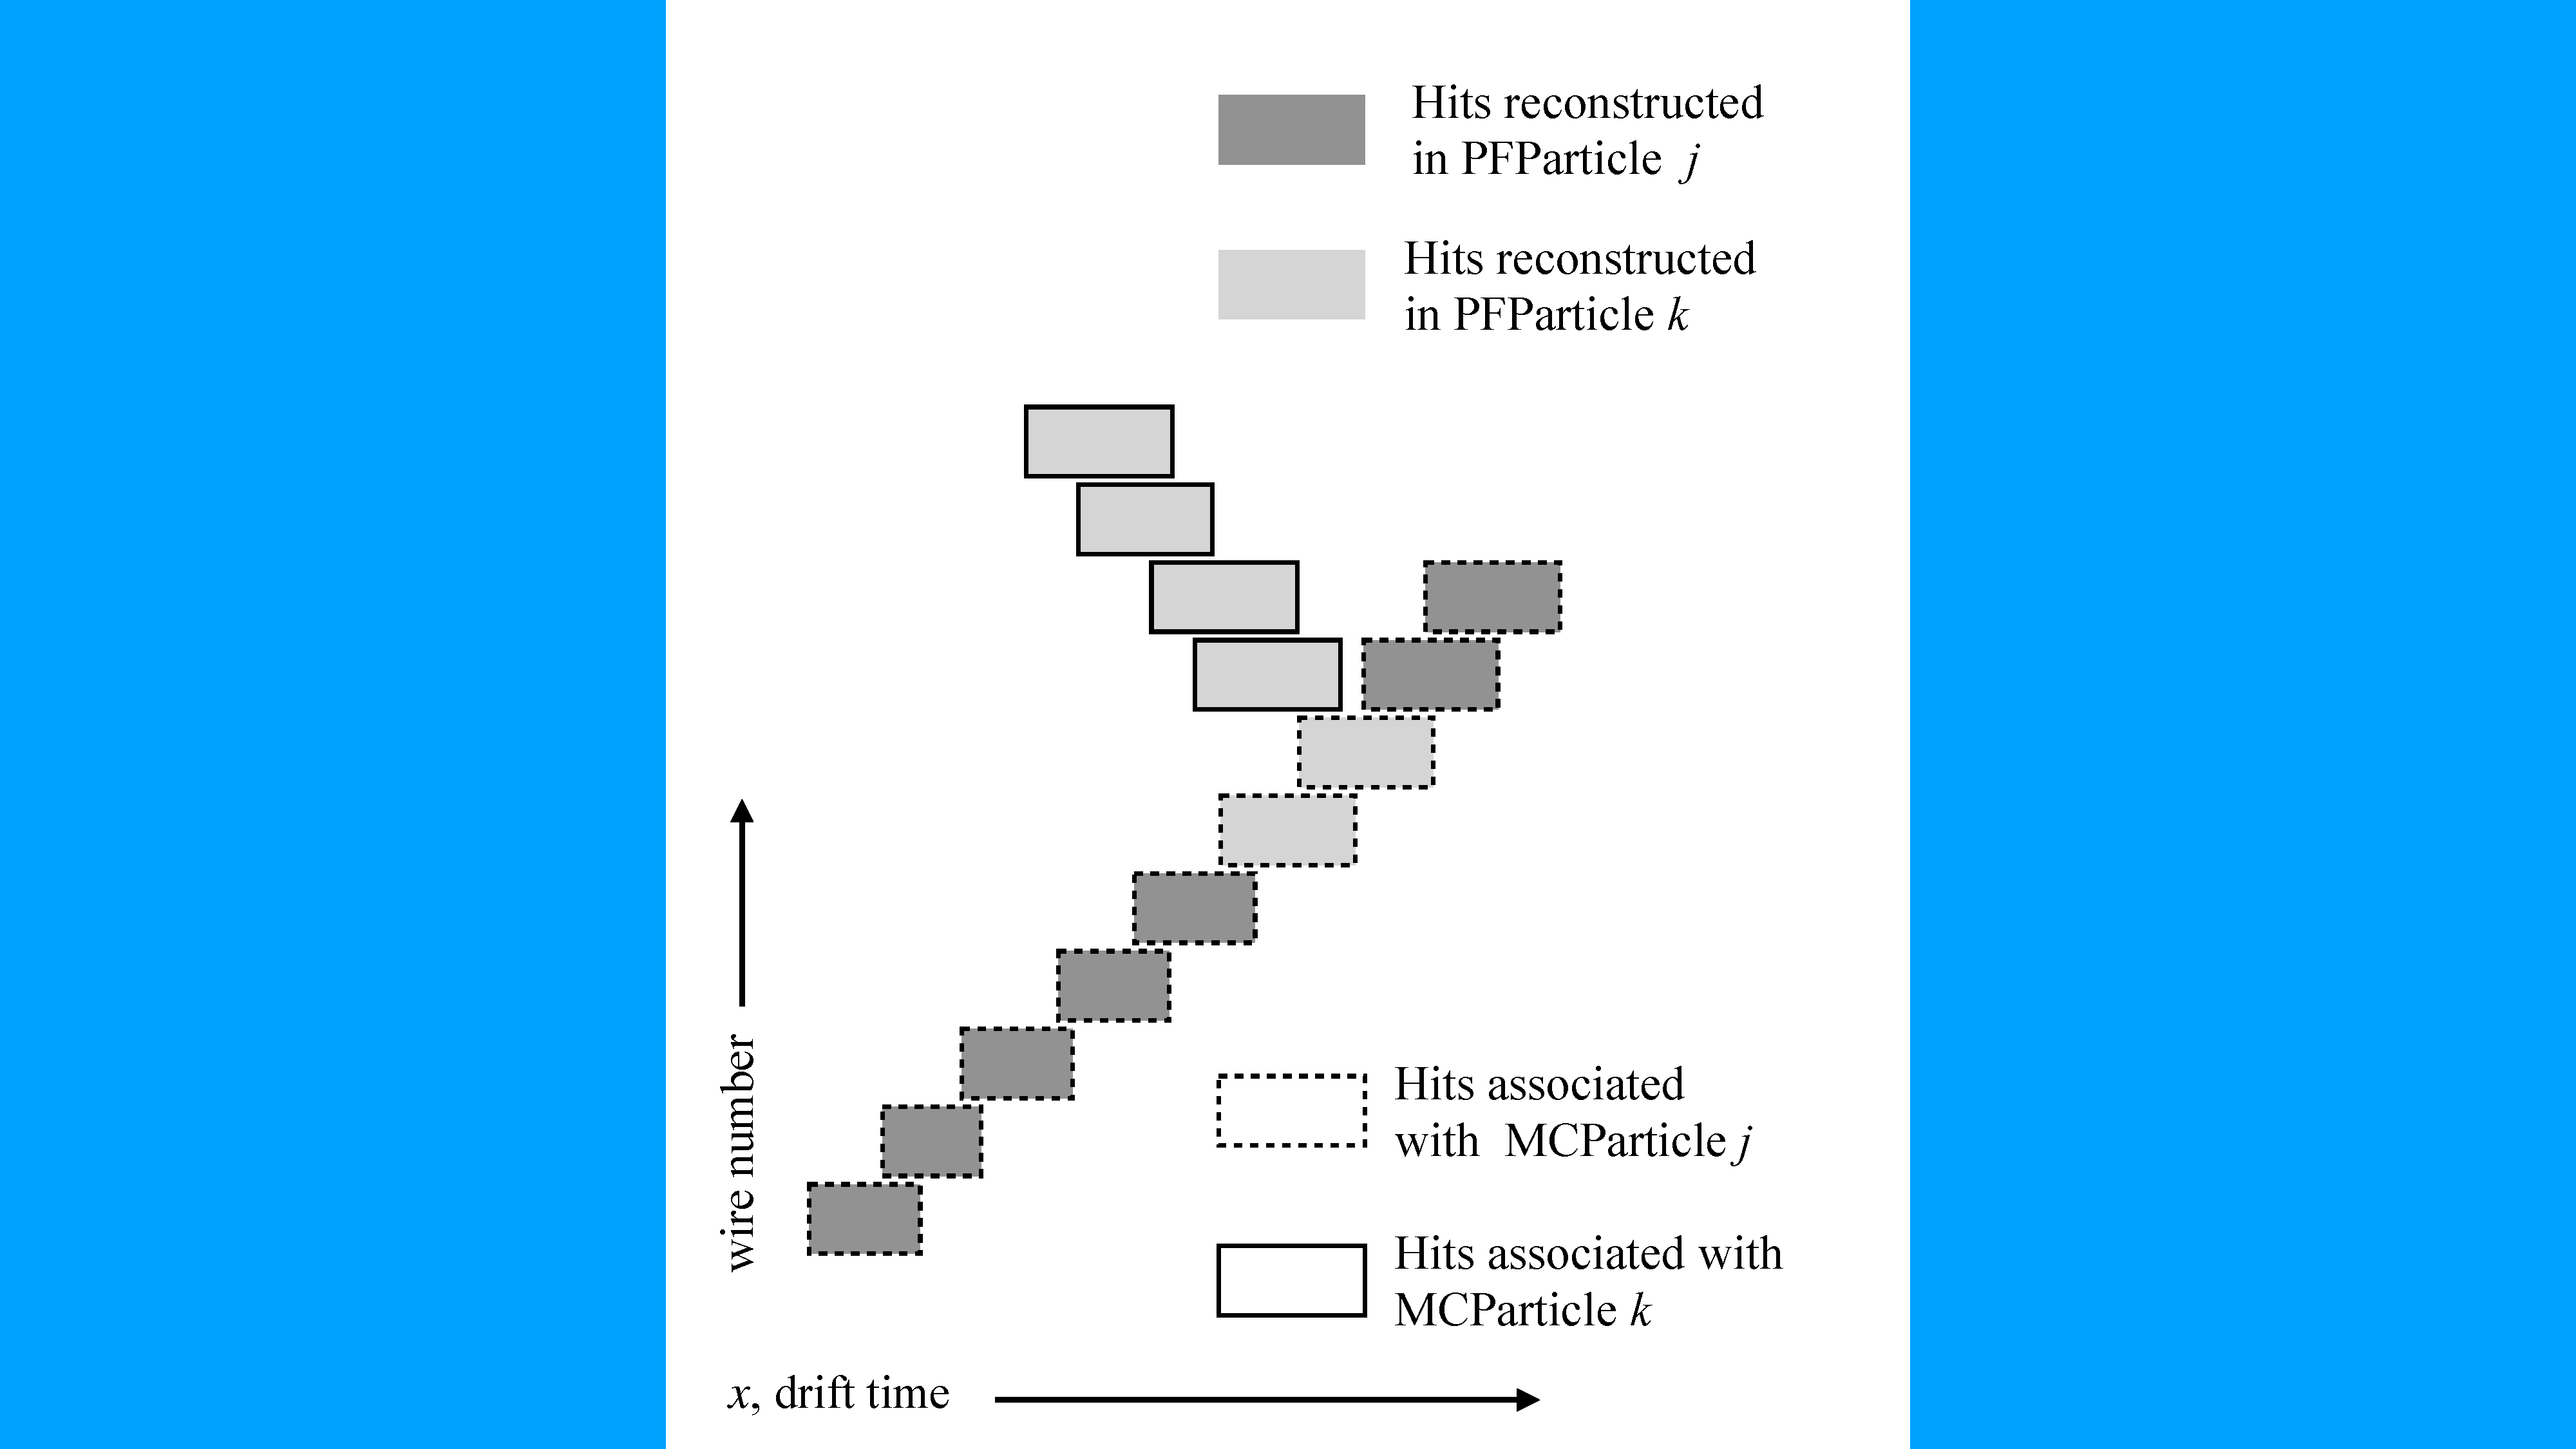
\includegraphics[width=0.5\linewidth, trim={18cm 0 18cm 0}, clip]{pandora/chapter_4/HIT_PUR_EFF.pdf}};
        \node[] at (6, 0) {
        \begin{minipage}[b]{5cm}
            \begin{tabular}{ccc}
                & Particle $j$ & Particle $k$ \\
                $\mathrm{hits_{MCParticle}}$ & 9 & 4 \\
                $\mathrm{hits_{PFParticle}}$ & 7 & 6 \\
                Matched hits & 7 & 4 \\
                Purity & 1 & 0.667 \\
                Completeness & 0.778 & 1
            \end{tabular}
        \end{minipage}
        };
    \end{tikzpicture}
    
    \caption[Definition of hit purity and completeness]{Illustration closeup of the MC hits with their association to both the true MCParticle (indicated by the border style) and the Pandora reconstructed PFParticle (indicated by the fill color). More detail is found in the text. }
    \label{fig:hit_pur_eff}
\end{figure}

Having provided the definition of hit purity and hit completeness, it is interesting to look at the effect of the CheatingClusterCreation algorithm in terms of hit purity and hit completeness. \autoref{fig:hit_purity_completeness_CCC} illustrate both the hit purity an the hit completeness for a sample of $1\PGm N\Pp$ selected using the true signal definition \cite{artero_pons_2024_13841852}, for both the protons and the muons involved in the process. Both the hit purity and hit completeness spectra show a preference for the higher part of the spectra in the case of the CheatedClusterCreation algorithm. 

Even though the cheated spectra show a improvement, there is a non-zero fraction of events for which the muon completeness is lower than \num{0.4}. 

\begin{figure}
    \centering
    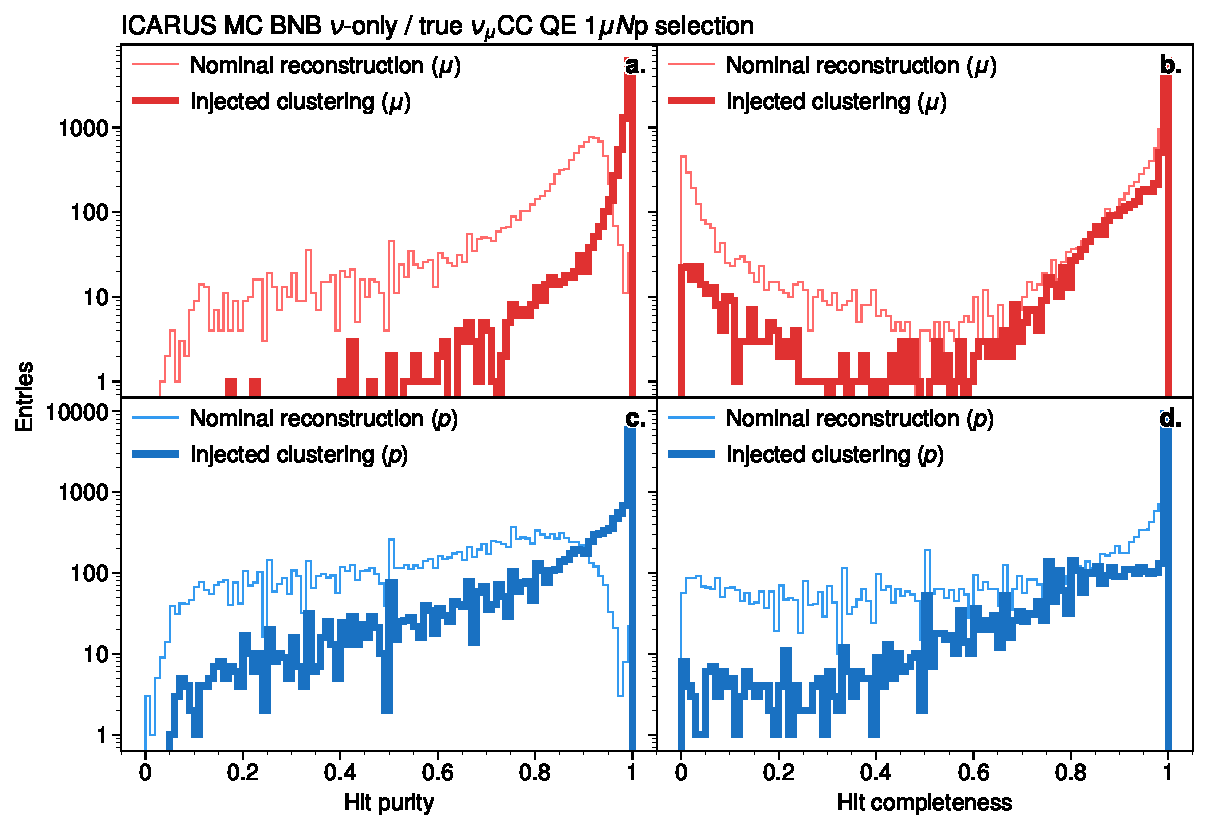
\includegraphics[width=0.95\linewidth]{pandora/chapter_4/toSlide_completeness_purity.pdf}
    \caption[Hit purity and completeness with CheatingClusterCreation algorithm]{Hit purity and hit completeness spectra for the proton (blue) and muon (red) population, for both the cheated cluster reconstruction (thick line) and the nominal reconstruction (thin line). }
    \label{fig:hit_purity_completeness_CCC}
\end{figure}

\subsection{Three-dimensional vertex}

There are two way true information can be used to inform the reconstruction of the interaction vertex. 

The straight-forward mode is to replace both the created vertex candidates and the selected interaction vertex with the the true $(x,y,z)$ position of the vertex as generated by Monte Carlo simulation. This operation is performed by the CheatingVertexCreation algorithm that replace all the vertex creation and selection algorithms in the XML steering configuration. 

\begin{figure}
    \centering
    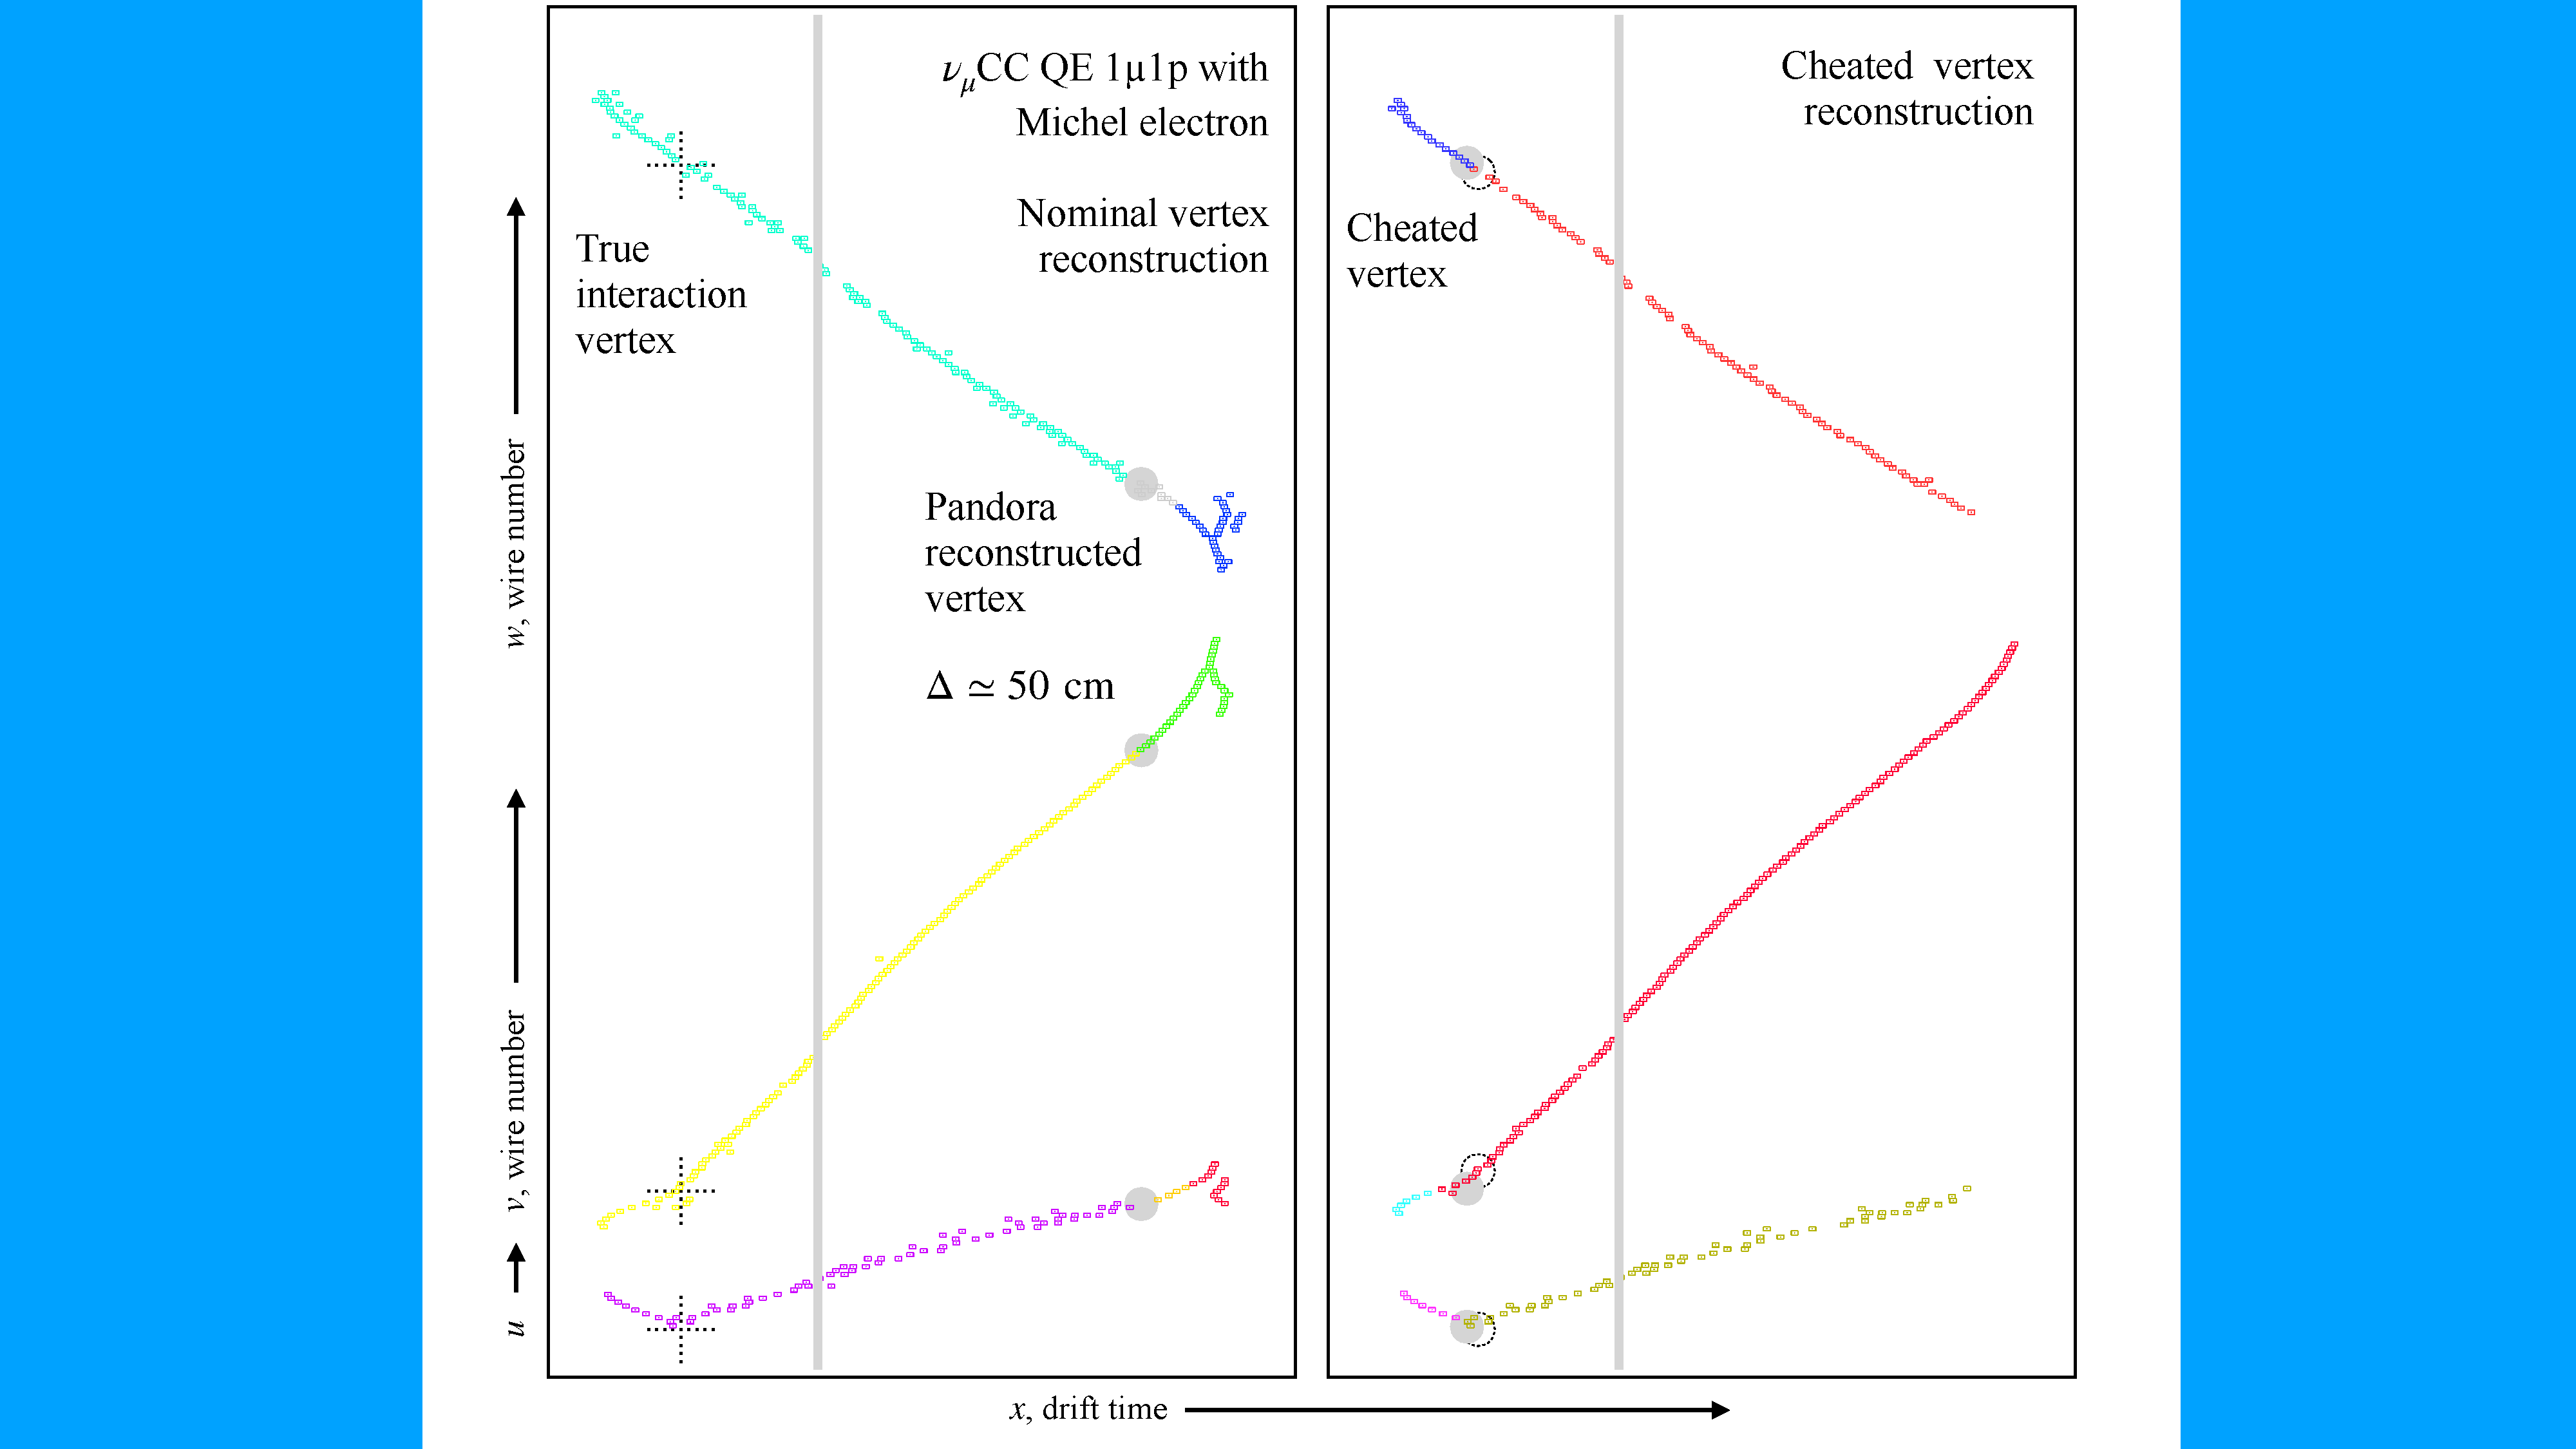
\includegraphics[width=0.95\linewidth, trim={12cm 0 11cm 0}, clip]{pandora/chapter_4/vertex.pdf}
    \caption[CheatingVertexCreation and CheatingVertexSelection algorithms]{}
    \label{fig:CheatingVertexCreation}
\end{figure}

\autoref{fig:CheatingVertexCreation} shows an example of one event where 


{\color{red} Some words on 1. injecting true vertex is not that safe (example of OoFV vertex), 2. true vertex $\neq$ reco vertex even in some cases $\to$ is the first hit reconstructed nearby? 3. other considerations?}


\begin{figure}
    \centering
    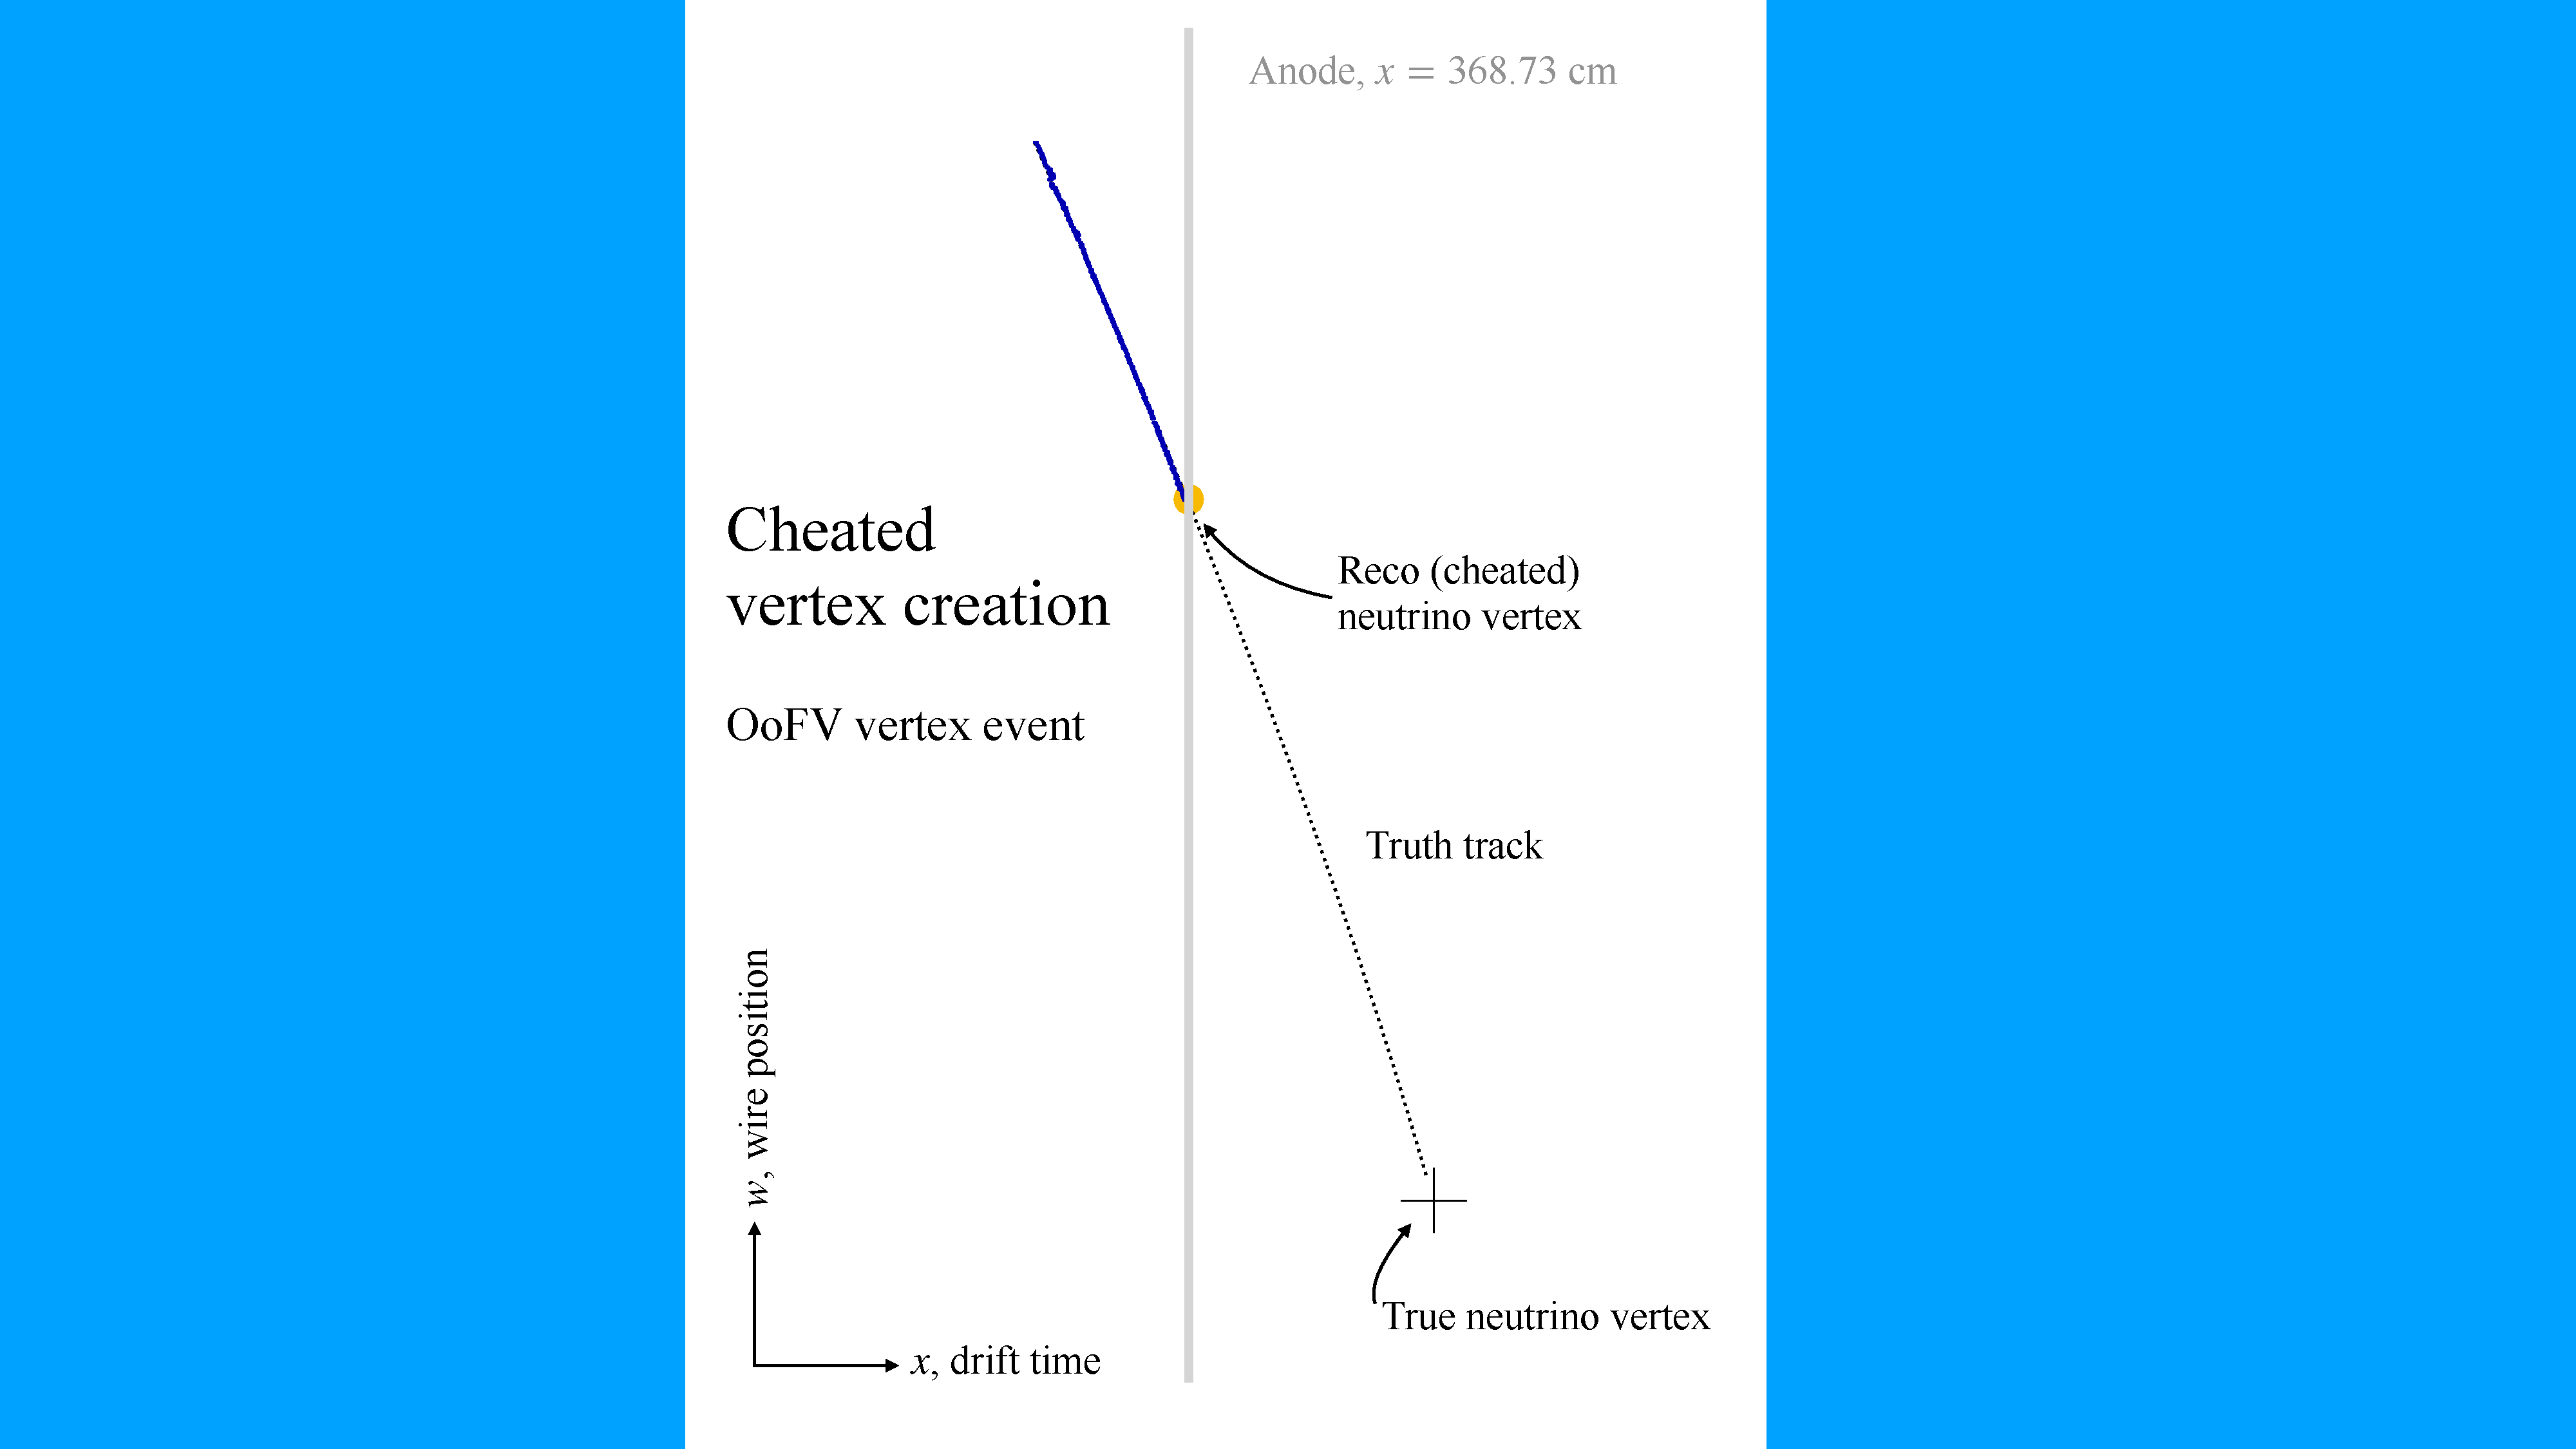
\includegraphics[width=0.55\linewidth, trim={18.5cm 0 22cm 0}, clip]{pandora/chapter_4/vertex_OoFV.pdf}
    \caption[CheatingVertexCreation with an OoFV vertex]{}
    \label{fig:CheatingVertexCreation}
\end{figure}

A second point where the true Monte Carlo information can be used to inform the vertex aglorithms is in the selection of the correct interaction vertex from the list of candidates created by the nominal CandidateVertexCreation algorithm. This operation is essentially bypassing the BdtVertexSelection algorithm and selecting, from the list of vertex candidates created as described in \autoref{sec:PandoraNeutrino}, the vertex which lies closest to the true interaction vertex based on a three-dimensional distance metric alone. 
{\color{red} Missing image. Show here the effects of the cheating and a metric valid to check it is working or later?}

\begin{figure}
    \centering
    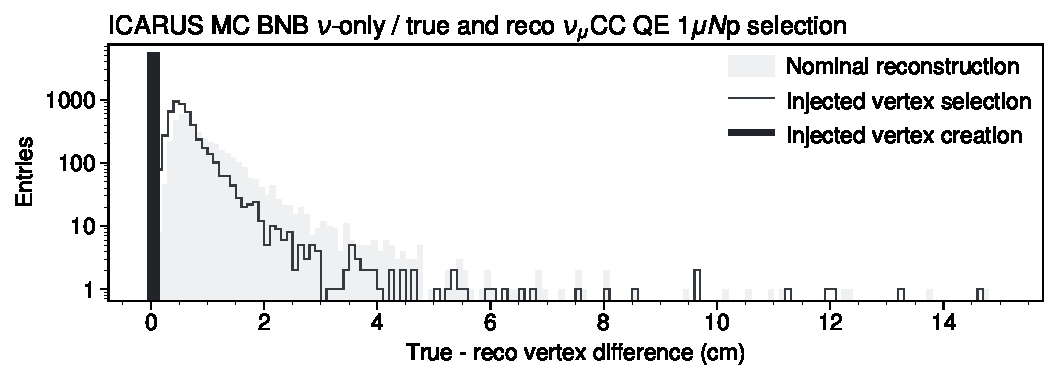
\includegraphics[width=\linewidth]{pandora/chapter_4/toSlide_vertexStudy.pdf}
    \caption[Vertex displacement from truth]{Displacement of the reconstructed vertex from the true vertex, computed when performing the nominal vertex recosntruction (shaded area), cheating the vertex selection (thin black line) and cheating the vertex creation algortithm (thick black line). }
    \label{fig:enter-label}
\end{figure}


\subsection{Three-dimensional track and shower reconstruction}

Like the other steps in the reconstruction, cheating the three-dimensional reconstruction steps follows from the nominal version of the algorithm. The idea is that a cheated version of a reconstruction step should replace the nominal version in the chain. This is why the cheating of the three-dimensional reconstruction stage is made of a cheated step, namely the CheatingPfoCreation algorithm, followed by the same ThreeDHitCreation algorithm employed in the nominal version of the reconstruction. In fact, event though the interaction is generated in three-dimensional space, the simulation of the hits is performed only on the 2D readout planes, so there is no possibility to really inject the true $(x,y,z)$ position of each hit, since it is not known. 

The CheatingPfoCreation algorithm goes through all the 2D clusters created by upstream stages of the reconstruction to identify those from each view that share the same true MCParticle. This operation is performed, similarly to the CheatingClusterCreation algorithm, exploiting the MCweight associated with the hits in the cluster. Clusters sharing more than \SI{50}{\percent} of the weighted hits with a given MCParticle are added together. 


\subsection{Particle hierarchy reconstruction}



\subsection{Particle classification}


\subsection{Slice }



\section{Evaluating subsequent reconstruction stages}



\section{Impact of the vertex reconstruction}

